\documentclass[../main/main.tex]{subfiles}

\newdate{date}{04}{11}{2020}

% \begin{figure}[h!]
% \centering
% \includegraphics[page=6,width=0.8\textwidth]{../lessons/pdf_file/14_lecture.pdf}
% \end{figure}

%\displaydate{date}. Compiled:  \today. Alice.

\begin{document}

\pagestyle{plain}

\section{Lecture 14}


\subsubsection*{Slide 1}

\begin{minipage}[]{0.5\linewidth}
\centering
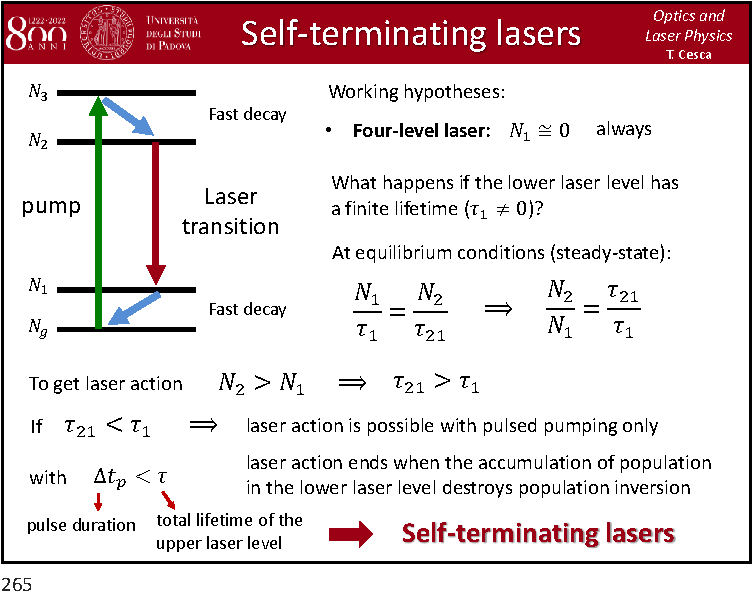
\includegraphics[page=1,width=1\textwidth]{../lessons/pdf_file/14_lecture.pdf}
\end{minipage}
\hspace{0.3cm}\vspace{0.3cm}
\begin{minipage}[c]{0.47\linewidth}

What happens if instead the lower laser laser as a lifetime different from zero?

Firstly, let us consider the steady-state condition: the number of spontaneous emission transition from the lower laser level is equal to the one of spontaneous trasmission from upper to lower state level.

In order to get laser action, we have to get population inversion which can be rewritten in terms of lifetimes.

Let us suppose that \( \tau _{21} < \tau _1 \): we can still get laser action by only by using pulsed pumping.

We need to work in a condition in which the \textbf{pulse duration} is lower than the \textbf{total lifetime of the upper laser level} to get laser action.

\end{minipage}

These kind of system which are able to stop laser action are called \textbf{self-terminating lasers}.

\subsubsection*{Slide 2}

\begin{minipage}[]{0.5\linewidth}
\centering
\includegraphics[page=2,width=1\textwidth]{../lessons/pdf_file/14_lecture.pdf}
\end{minipage}
\hspace{0.3cm}\vspace{0.3cm}
\begin{minipage}[c]{0.47\linewidth}

Let us make some exercises in order to apply the expressions for the CW system.

\end{minipage}

\subsubsection*{Slide 3}

\begin{minipage}[]{0.5\linewidth}
\centering
\includegraphics[page=3,width=1\textwidth]{../lessons/pdf_file/14_lecture.pdf}
\end{minipage}
\hspace{0.3cm}\vspace{0.3cm}
\begin{minipage}[c]{0.47\linewidth}

Let us find the \textbf{photon lifetime}.

\end{minipage}

\newpage

\subsubsection*{Slide 4}

\begin{minipage}[]{0.5\linewidth}
\centering
\includegraphics[page=4,width=1\textwidth]{../lessons/pdf_file/14_lecture.pdf}
\end{minipage}
\hspace{0.3cm}\vspace{0.3cm}
\begin{minipage}[c]{0.47\linewidth}

Compute the \textbf{number of photons in the cavity} trough the expression of the output power.

\end{minipage}

\subsubsection*{Slide 5}

\begin{minipage}[]{0.5\linewidth}
\centering
\includegraphics[page=5,width=1\textwidth]{../lessons/pdf_file/14_lecture.pdf}
\end{minipage}
\hspace{0.3cm}\vspace{0.3cm}
\begin{minipage}[c]{0.47\linewidth}

Compute the \textbf{critical population inversion}.

Finally, let us compute the \textbf{saturation intensity} (we are in the gain condition).

A very small fraction of the total population is used.

\end{minipage}

\subsubsection*{Slide 6}

\begin{minipage}[]{0.5\linewidth}
\centering
\includegraphics[page=6,width=1\textwidth]{../lessons/pdf_file/14_lecture.pdf}
\end{minipage}
\hspace{0.3cm}\vspace{0.3cm}
\begin{minipage}[c]{0.47\linewidth}

Let us consider another example of laser: the \textbf{He-Ne laser}. Globally, this system can be though as a four-level system.

\end{minipage}

\newpage

\subsubsection*{Slide 7}

\begin{minipage}[]{0.5\linewidth}
\centering
\includegraphics[page=7,width=1\textwidth]{../lessons/pdf_file/14_lecture.pdf}
\end{minipage}
\hspace{0.3cm}\vspace{0.3cm}
\begin{minipage}[c]{0.47\linewidth}

Let us solve the same problem with the He-Ne laser.

\end{minipage}

\subsubsection*{Slide 8}

\begin{minipage}[]{0.5\linewidth}
\centering
\includegraphics[page=8,width=1\textwidth]{../lessons/pdf_file/14_lecture.pdf}
\end{minipage}
\hspace{0.3cm}\vspace{0.3cm}
\begin{minipage}[c]{0.47\linewidth}

\end{minipage}

\subsubsection*{Slide 9}

\begin{minipage}[]{0.5\linewidth}
\centering
\includegraphics[page=9,width=1\textwidth]{../lessons/pdf_file/14_lecture.pdf}
\end{minipage}
\hspace{0.3cm}\vspace{0.3cm}
\begin{minipage}[c]{0.47\linewidth}

We have a much lower output power for this system. In this case the cavity is completely filled with the active medium.

\end{minipage}

\subsubsection*{Slide 10}

\begin{minipage}[]{0.5\linewidth}
\centering
\includegraphics[page=10,width=1\textwidth]{../lessons/pdf_file/14_lecture.pdf}
\end{minipage}
\hspace{0.3cm}\vspace{0.3cm}
\begin{minipage}[c]{0.47\linewidth}

\end{minipage}

\subsubsection*{Slide 11}

\begin{minipage}[]{0.5\linewidth}
\centering
\includegraphics[page=11,width=1\textwidth]{../lessons/pdf_file/14_lecture.pdf}
\end{minipage}
\hspace{0.3cm}\vspace{0.3cm}
\begin{minipage}[c]{0.47\linewidth}

As said, the behavior in CW mode can be summarized as in this graph.

Let us assuming a constant pumping rate and constant losses.

In the condition below treshold the population inversion increase with an exponential form and reach an asymptotic value.

The fact that we are above or below treshold depends on the losses inside the cavity. As said, the larger are the losses the smaller is the photon lifetime. We can introduce the \textbf{quality factor}.

Let us suppose that at a given instant we can reduce the losses inside the cavity. Hence, we are changing the \( Q \) factor from a low value (high losses) to a high value (low losses). This is a \textbf{Q-switch}: we are switching the losses from high value to low value.
\end{minipage}

All the population inversion accumulated in the medium while the losses are high are immediatly transferred to the cavity. We obtain a huge transfer of energy from active medium to the cavity. We will produce a large number of photon in the cavity in a short time: the \textbf{emission will be pulsed} of the order of few ns.

\subsubsection*{Slide 12}

\begin{minipage}[]{0.5\linewidth}
\centering
\includegraphics[page=12,width=1\textwidth]{../lessons/pdf_file/14_lecture.pdf}
\end{minipage}
\hspace{0.3cm}\vspace{0.3cm}
\begin{minipage}[c]{0.47\linewidth}

The Q-switch is a mode in order to produce pulsed emission with time emission of the order of ns: we first accumulate energy in the active medium by pumping the system in a situation in which the system is not able to give laser action (below treshold). Then, we immediately switch the cavity \( Q \) factor and all the accumulated energy will be transferred to the cavity.

We will describe the \textbf{active} Q-switch in which the change of the \( Q \) factor is obtained with an active system. For instance, by introducing a shutter in a cavity which if is close accumulate energy. Then, you open the shutter and you will get laser action with the formation of the pulse.

Then, we consider a \textbf{fast} Q-switch: the transition from low to high losses is instantaneous.

The last hypothesis is that we consider \textbf{pulsed pumping}. We stop the pumping in the moment in which we open the shutter and in which we switch the \( Q \) factor.

\end{minipage}


\subsubsection*{Slide 13}

\begin{minipage}[]{0.5\linewidth}
\centering
\includegraphics[page=13,width=1\textwidth]{../lessons/pdf_file/14_lecture.pdf}
\end{minipage}
\hspace{0.3cm}\vspace{0.3cm}
\begin{minipage}[c]{0.47\linewidth}

The duration of the pump pulse needs to be smaller than the lifetime of the upper laser level. If we pump the system for longer times than the upper laser level, the population inversion reach the asymptotic value \( N_{\infty } \): the pump power will be lost by spontaneous decay instead of being accumulated. According to \( N_{\infty } \), in order to accumulate larger population inversion we need to have a system with a longer lifetime \( \tau  \). This is why this is a mode commonly used for solid state medium or for instance Erbium is used. For gas lasers the lifetime of the upper laser is not too high. That is why you will never see He-Ne laser working in Q-switch mode. Hence, the reason is how much population inversion you can get before the system is in laser action.

\end{minipage}

\subsubsection*{Slide 14}

\begin{minipage}[]{0.5\linewidth}
\centering
\includegraphics[page=14,width=1\textwidth]{../lessons/pdf_file/14_lecture.pdf}
\end{minipage}
\hspace{0.3cm}\vspace{0.3cm}
\begin{minipage}[c]{0.47\linewidth}

In CW mode we will consider \textbf{space-independent rate equations}. The hypothesis are reported here.

\end{minipage}

\subsubsection*{Slide 15}

\begin{minipage}[]{0.5\linewidth}
\centering
\includegraphics[page=15,width=1\textwidth]{../lessons/pdf_file/14_lecture.pdf}
\end{minipage}
\hspace{0.3cm}\vspace{0.3cm}
\begin{minipage}[c]{0.47\linewidth}

We will rewrite the very same equation which we wrote to describe the behavior in CW mode.

\( E_p \) is the \textbf{pump energy} proportional to the integral of the pumping rate. Hence, it can be considered proportional to the initial population inversion that we have.

\end{minipage}

\subsubsection*{Slide 16}

\begin{minipage}[]{0.5\linewidth}
\centering
\includegraphics[page=16,width=1\textwidth]{../lessons/pdf_file/14_lecture.pdf}
\end{minipage}
\hspace{0.3cm}\vspace{0.3cm}
\begin{minipage}[c]{0.47\linewidth}

We can rewrite the \textbf{over-threshold factor}: the ratio between the pumping energy and the critical pumping energy or can be written as the ratio between the initial population inversion and the critical population inversion.

The losses to consider \( N_c = \gamma / \sigma l  \) are the losses \( \gamma   \) when the shutter is open! So, when we have made the Q-switch!
This is a very important point!

We can use these relationships to solve the rate equations.
\end{minipage}


\subsubsection*{Slide 17}

\begin{minipage}[]{0.5\linewidth}
\centering
\includegraphics[page=17,width=1\textwidth]{../lessons/pdf_file/14_lecture.pdf}
\includegraphics[page=18,width=1\textwidth]{../lessons/pdf_file/14_lecture.pdf}
\end{minipage}
\hspace{0.3cm}\vspace{0.3cm}
\begin{minipage}[c]{0.47\linewidth}

Since we are considering that the Q-switch is fast, the temporal evolution of the population inversion and of the number of photon in the cavity occurs in a time range that so short that we can neglect it in the first rate equation the term related to the pumping rate and the spontaneous decay.   

\end{minipage}




\end{document}
